\section{Systems with zeros}\label{sec:zeros}

The main theorem concerns zero-free systems. A passive system may also have
zeros in $\Cp$, and a zero contributes phase without contributing loss on
the real axis. This section shows that zeros do help, and by how much one
zero helps.

\subsection{The bound with an inner factor}

\begin{proposition}\label{prop:inner}
Let $H=BG$ be passive, where $B$ is a real-symmetric Blaschke product whose
zeros stay away from $I\cup(-I)$ and $G$ is zero-free and regular on the
band. Let $\varphi$ be a continuous argument of $H$ on $[a,b]$ and let $\psi$
be the continuous argument of $B$ on $[a,b]$ for which $\varphi-\psi$ is the
phase of $G$ in the sense of \cref{lem:log}. Then $\alpha=\alpha_G$ on the
band, and
\begin{equation}\label{eq:inner}
\begin{aligned}
\int_a^b\alpha\dd\omega&=\frac12\int_a^b(\varphi-\psi)\,p\dd\omega
+\frac\pi4\int_{\R\setminus S}W\dd\mu_G\\
&\ge\ \frac12\int_a^b(\varphi-\psi)\,p\dd\omega .
\end{aligned}
\end{equation}
The function $\psi$ is real-analytic and strictly increasing on $[a,b]$.
\end{proposition}

\begin{proof}
The Blaschke product is analytic across $I$ and unimodular there, so
$\log\abs H=\log\abs G$ on the band, and $\arg H=\arg B+\arg G$ modulo $2\pi$.
The continuous arguments on $[a,b]$ therefore differ by a constant in
$2\pi\Z$, which fixes $\psi$. \Cref{thm:sumrule} applied to $G$ gives
\eqref{eq:inner}. The monotonicity of $\psi$ is the computation in the
proof of \cref{prop:foster}.\footnote{For a single factor
$(z-\zeta)/(z-\bar\zeta)$ with $\zeta=\xi+i\eta$, $\eta>0$, the argument on the
real line is $\arg(x-\zeta)-\arg(x-\bar\zeta)$, and
$\frac{\dd}{\dd x}\arg(x-\xi\mp i\eta)=\pm\eta/((x-\xi)^2+\eta^2)$; the
difference is $2\eta/\abs{x-\zeta}^2$.}
\end{proof}

An increasing $\psi$ behaves like a delay distributed over frequency. A pure
delay is free (\cref{lem:moments}(i)), but a phase that rises steeply at low
frequencies and flattens on the band is not a delay: its weighted integral
$\int\psi p$ is positive, and \eqref{eq:inner} then allows less loss than
\eqref{eq:main}. The simplest instance is a single zero on the imaginary
axis.

\subsection{One zero}

For $\eta>0$ let
\[
B_\eta(z)=\frac{z-i\eta}{z+i\eta}.
\]
It is passive, unimodular on $\R$, has the real symmetry, and the argument
of $-B_\eta$ on $(0,\infty)$ is
\begin{equation}\label{eq:Bphase}
\arg\big(-B_\eta(\omega)\big)=\pi-2\arctan\frac\eta\omega=2\arctan\frac\omega\eta
\in(0,\pi).
\end{equation}
For $0<\theta<\pi$ put $\eta_\theta=b\cot(\theta/2)$, so that
$2\arctan(b/\eta_\theta)=\theta$.

\begin{proposition}\label{prop:onezero}
Let $0<\theta<\pi$ and $\eta\ge\eta_\theta$, and put
\[
g_\eta(\omega)=\theta-2\arctan\frac\omega\eta,\qquad
H_\eta=-B_\eta\,e^{ih_{g_\eta}},
\]
with $h_g$ as in \cref{prop:profile}. Then $H_\eta$ is passive and regular on
the band, has exactly one zero in $\Cp$, at $i\eta$, has argument $\theta$
on $[a,b]$, and
\begin{equation}\label{eq:onezero}
\begin{gathered}
\frac1{b-a}\int_a^b\alpha_\eta\dd\omega=\theta\Lambda-\delta(\eta),\\
\delta(\eta)=\frac1{b-a}\int_a^b\arctan\frac\omega\eta\,p(\omega)\dd\omega .
\end{gathered}
\end{equation}
The reduction $\delta$ is strictly positive and strictly decreasing in $\eta$,
and
\begin{equation}\label{eq:delta-asym}
\delta(\eta)=\frac{\pi(b^2-a^2)^2}{24(b-a)\eta^3}+O(\eta^{-5})\qquad(\eta\to\infty).
\end{equation}
\end{proposition}

\begin{proof}
On $[a,b]$ the function $g_\eta$ is decreasing, and $g_\eta(b)\ge0$ because
$\eta\ge\eta_\theta$. Hence $g_\eta\ge0$, $g_\eta>0$ on $[a,b)$, and
$g_\eta(t)/t$ is decreasing. By \cref{lem:positivity}, $v_{g_\eta}\ge0$ and
$\beta_{g_\eta}>0$, so by \cref{prop:profile}(iii) $e^{ih_{g_\eta}}$ is a
zero-free passive system, regular on the band, with phase $g_\eta$ and
attenuation $v_{g_\eta}$, and with no measure outside $S$. Multiplying by
$-B_\eta$ keeps passivity and the real symmetry, adds the single zero $i\eta$,
leaves the modulus on $\R$ unchanged, and adds the argument
\eqref{eq:Bphase}. The argument of $H_\eta$ on the band is therefore
$g_\eta+2\arctan(\omega/\eta)=\theta$, and \cref{prop:profile}(iii) gives
\[
\int_a^b\alpha_\eta=\frac12\int_a^bg_\eta\,p=\frac\theta2J-\int_a^b\arctan\frac\omega\eta\,p\dd\omega,
\]
which is \eqref{eq:onezero} since $J=2(b-a)\Lambda$.

For the sign, write $\arctan(x/\eta)=x\,f(x^2)$ with
$f(\sigma)=\arctan(\sqrt\sigma/\eta)/\sqrt\sigma$. Since $u\mapsto\arctan(u)/u$
is strictly decreasing on $(0,\infty)$,\footnote{Its derivative is
$\big(u/(1+u^2)-\arctan u\big)/u^2$, and $\arctan u>u/(1+u^2)$ for $u>0$ because
both vanish at $0$ and $\frac{\dd}{\dd u}\arctan u=\frac1{1+u^2}>
\frac{1-u^2}{(1+u^2)^2}=\frac{\dd}{\dd u}\frac u{1+u^2}$.} $f$ is strictly
decreasing, and \cref{lem:moments}(ii) gives $\delta(\eta)>0$. Similarly
\[
\delta'(\eta)=-\frac1{b-a}\int_a^b\frac{x\,p(x)}{\eta^2+x^2}\dd x<0,
\]
by \cref{lem:moments}(ii) with the strictly decreasing
$f(\sigma)=1/(\eta^2+\sigma)$. Finally
$\arctan u=u-u^3/3+O(u^5)$ uniformly on $[0,b/\eta]$, and
\cref{lem:moments}(i),(iv) give $\int_a^bx\,p=0$ and
$\int_a^bx^3p=-\frac\pi8(b^2-a^2)^2$, which yields \eqref{eq:delta-asym}.
\end{proof}

Since $\delta$ decreases, the best choice within the family is
$\eta=\eta_\theta$, where the phase $g_\eta$ of the zero-free factor reaches
zero at the upper band edge. \Cref{fig:zero} shows the mean loss of
$H_\eta$, relative to $\theta\Lambda$, over $\theta$ and $\eta/\eta_\theta$.

\begin{figure}[t]
\centering
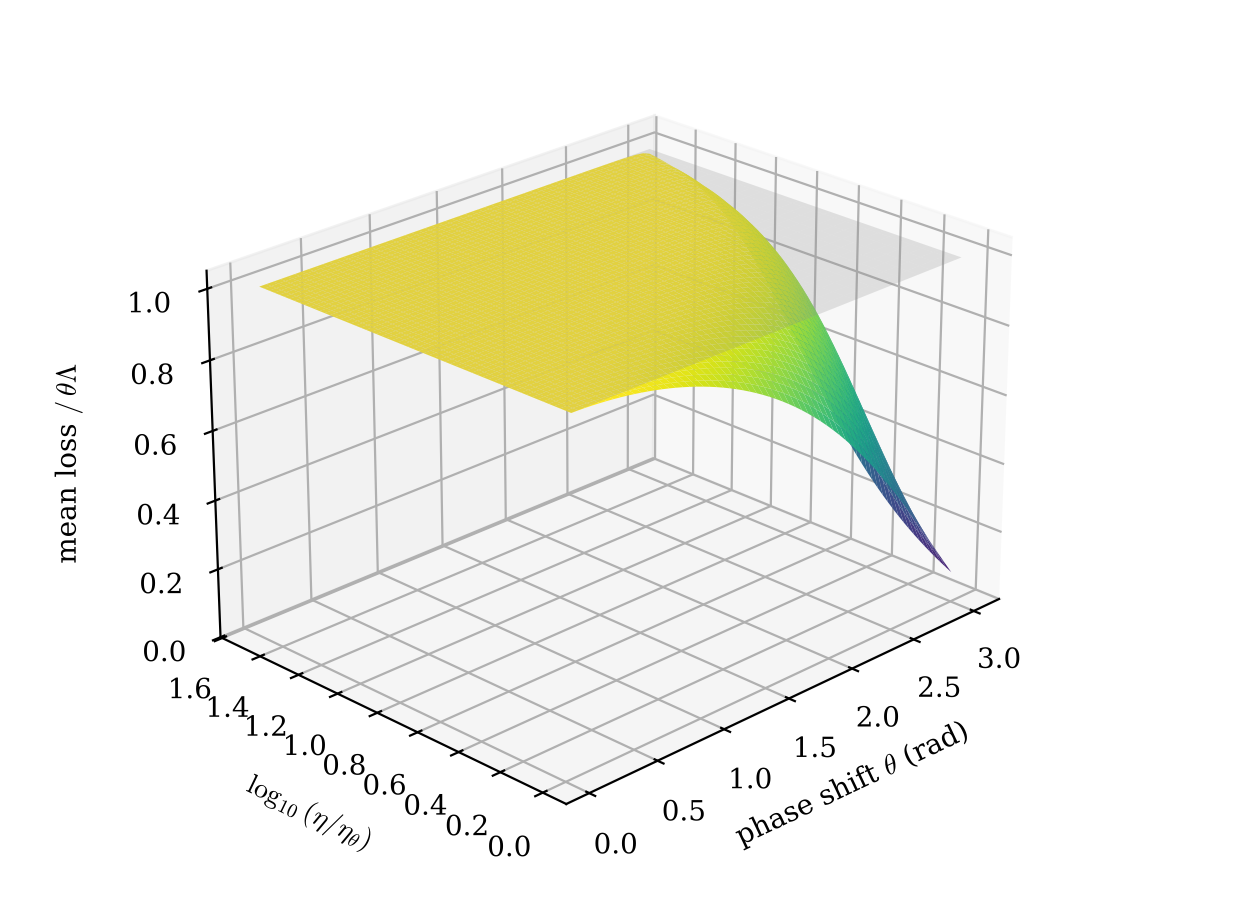
\includegraphics[width=\columnwidth]{figures/fig_zero.png}
\caption{The mean attenuation of the one-zero system $H_\eta$ of
\cref{prop:onezero}, divided by the zero-free bound $\theta\Lambda$, for
$a=1$, $b=2$, over the phase $\theta$ and $\log_{10}(\eta/\eta_\theta)$. The
grey plane is the level $1$. The ratio is below $1$ everywhere and tends to
$1$ as the zero moves to infinity.}
\label{fig:zero}
\end{figure}

\subsection{One zero beats every zero-free system}

The statement of \cref{thm:main} fixes the continuous phase $\varphi$. A
measurement only gives the argument modulo $2\pi$, and a zero-free system
with $\arg H\equiv\theta$ may realise $\theta$ through a lead $\theta-\pi$, by
\cref{rem:arg}. The next corollary takes this into account.

\begin{corollary}\label{cor:zerosbeat}
Let $0<\theta<a\pi/(a+b)$. Among zero-free passive systems regular on the
band with $\arg H\equiv\theta$ modulo $2\pi$ on $[a,b]$, the least mean
attenuation over the band is $\theta\Lambda$, attained by $H_\star$. The
system $H_{\eta_\theta}$ of \cref{prop:onezero}, which has one zero, has the
same argument and a strictly smaller mean attenuation.
\end{corollary}

\begin{proof}
By \cref{rem:arg} the phase of such a system is a constant $\theta'$ with
$\theta'\equiv\theta\pmod\pi$. If $\theta'\ge\theta$, \cref{thm:main} gives
mean attenuation at least $\theta'\Lambda\ge\theta\Lambda$. Otherwise
$\theta'\le\theta-\pi<0$, and \cref{thm:lead} with $\tau=0$ bounds the
$ab/\omega^2$-weighted mean by $\abs{\theta'}\Lambda\ge(\pi-\theta)\Lambda$.
Since $ab/\omega^2\le b/a$ on $[a,b]$, the plain mean is at least
$(a/b)(\pi-\theta)\Lambda$, which exceeds $\theta\Lambda$ exactly when
$\theta<a\pi/(a+b)$. The value $\theta\Lambda$ is attained by $H_\star$
(\cref{thm:extremal}), and \cref{prop:onezero} gives the second statement.
\end{proof}

For larger $\theta$ the lead branch competes. The system
$-H_\star(-ab/z)$, built from the extremal for $\pi-\theta$, is zero-free, has
$\sigma=-1$ and phase $\theta-\pi$, hence argument $\theta$ modulo $2\pi$, and
by \cref{rem:leadmean} its mean attenuation is
$(\pi-\theta)\,(E(\kappa)-\kappa'^2K(\kappa))/\kappa$. \Cref{tab:zeros} compares the
three systems for an octave.

\begin{table}[t]
\caption{Mean attenuation over the octave $[1,2]$ of three systems with
argument $\theta$ modulo $2\pi$: the lag extremal $H_\star$ (the least value
among zero-free systems with phase $\theta$), the lead extremal
$-H_\star(-ab/z)$ built for $\pi-\theta$, and the one-zero system
$H_{\eta_\theta}$. For $\theta<\pi/3$ the first column is the least value
among all zero-free systems (\cref{cor:zerosbeat}).}
\label{tab:zeros}
\centering
\small
\begin{tabular}{@{}rrrr@{}}
\toprule
$\theta$ & $\theta\Lambda$ & $(\pi-\theta)\,0.26560$ & $H_{\eta_\theta}$ \\
\midrule
$0.5$    & $0.13677$ & $0.70160$ & $0.13443$ \\
$1$      & $0.27353$ & $0.56880$ & $0.25394$ \\
$\pi/2$  & $0.42966$ & $0.41720$ & $0.34659$ \\
$2$      & $0.54707$ & $0.30320$ & $0.35977$ \\
$2.5$    & $0.68383$ & $0.17040$ & $0.27677$ \\
\bottomrule
\end{tabular}
\end{table}

The one-zero system is the best of the three for $\theta\le\pi/2$; by
$\theta=2$ the lead branch is better. For $\theta=0.5$ the zero lowers
the loss by $1.7\%$, for $\theta=1$ by $7.2\%$.

\subsection{The problem}

\begin{problem}\label{prob:zeros}
Determine
\[
\Lambda_{\mathrm{all}}(\theta)=\inf\Big\{\frac1{b-a}\int_a^b\alpha\dd\omega\Big\},
\]
the infimum over all passive systems $H$, with or without zeros, that are
continuous and nonzero near the band and satisfy $\arg H\equiv\theta$ modulo
$2\pi$ on $[a,b]$. Is $\Lambda_{\mathrm{all}}(\theta)>0$ for
$\theta\notin\pi\Z$?
\end{problem}

\Cref{cor:rigid} shows that the infimum is not attained by a lossless
system, but it does not exclude that it is zero. By \eqref{eq:inner}, the
question is how large $\int_a^b\psi\,p$ can be made by the argument $\psi$ of
a Blaschke product, while the remaining phase $\theta-\psi$ is still the
phase of a zero-free passive system. The difficulty is the second
condition: by \cref{prop:profile} it requires $v_g\ge0$ and $\beta_g\ge0$ for
$g=\theta-\psi$, and $\beta_g\ge0$ fails as soon as $g$ is too negative on the
band.\footnote{For instance, two zeros chosen so that $g<0$ on the whole band
give $\beta_g=\frac2\pi\int g/r<0$; the resulting function $e^{ih_g}$ grows
like $e^{-\beta_g y}$ along $i\R_+$ and is not passive.} The next section
solves the problem. The infimum is positive and attained, the minimiser has
exactly one zero, and it is the least lossy system at every frequency of the
band at once.
